\documentclass[12pt]{article}
\usepackage[T2A]{fontenc}
\usepackage[utf8]{inputenc}
\usepackage{multirow}
\usepackage{caption}
\usepackage{subcaption}
\usepackage{amsmath}
\usepackage{changepage}
\usepackage{graphicx}
\usepackage{float}
\usepackage[english,russian]{babel}
\usepackage{amsmath, amsfonts, amssymb, amsthm, mathtools}
\usepackage{xcolor}
\usepackage{array}
\usepackage{hyperref}
\usepackage[top = 1.5cm, left = 1.5 cm, right = 1.5 cm, bottom = 3 cm]{geometry}
\graphicspath{ {./images/} }
 
\title{Определение теплопроводности воздуха при атмосферном давлении}
\author{Шахматов Андрей, Б02-304}
\date{\today}
  
\begin{document}
\begin{titlepage}
    \begin{center}
        {\large МОСКОВСКИЙ ФИЗИКО-ТЕХНИЧЕСКИЙ ИНСТИТУТ (НАЦИОНАЛЬНЫЙ ИССЛЕДОВАТЕЛЬСКИЙ УНИВЕРСИТЕТ)}
    \end{center}
    \begin{center}
        {\large Физтех-школа физики и исследований им. Ландау}
    \end{center}
    
    
    \vspace{3cm}
    {\huge
        \begin{center}
            \textbf{Определение теплопроводности воздуха при атмосферном давлении}
        \end{center}
    }
    \vspace{2cm}
    \begin{flushright}
        {\LARGE Автор:\\ Шахматов Андрей Юрьевич \\
            \vspace{0.2cm}
            Б02-304}
    \end{flushright}
    \vspace{7 cm}
    \begin{center}
        Долгопрудный 2024
    \end{center}
\end{titlepage}

% \maketitle

\begin{abstract}
    Исследована зависимость теплопроводности воздуха в диапазоне темпператур \(20 - 80\) \textcelsius. Получена эмперическая 
    зависимость коэффициента теплопроводности \(\kappa \) от температуры \(T\): \(\kappa = A T\).    
\end{abstract}

\tableofcontents

\section{Введение}
Цель настоящей работы заключалась в определении коэффициента теплопроводности воздуха при различных температурах.

\section{Методика}
\subsection{Теоретическая справка}
В эксперименте будет измеряться коэффициент теплопроводности $\kappa$ - константа, фигурирущая в законе Фурье: 
\begin{equation}
    \vec{q} = -\kappa \nabla T, 
    \label{eq:1}
\end{equation} 
где $\vec{q}$ - количество теплоты переносимое через единичную площадку в единицу времени. 
Согласно \cite{Kirichenko} существует оценка для теплопроводности газов через длину свободного пробега молекул $\lambda$, 
среднюю скорости теплового движения $\overline{v} = \sqrt{\frac{8kT}{\pi m}}$, концентрацию $n$ и теплоёмкость при постоянном объёме в расчёте на одну молекулу $c_v$: 
\begin{equation}
    k \sim \lambda \overline{v} n c_v.
    \label{eq:2}
\end{equation}
С учётом оценки длины пробега $\lambda = \frac{1}{n\sigma}$ получим ожидаемую зависимость 
теплопроводности от температуры:
\begin{equation}
    k \propto \frac{\overline{v}}{\sigma} \propto \sqrt{T} 
\end{equation} 
Последний переход справедлив для модели твёрдых шариков ($\sigma = const$).
\subsection{Геометрия задачи}
Для измерения теплоёмкости было решено использовать простейший геометрический случай - циллиндрический (Рис. \ref{fig:1}).
\begin{figure}[H]
    \centering
    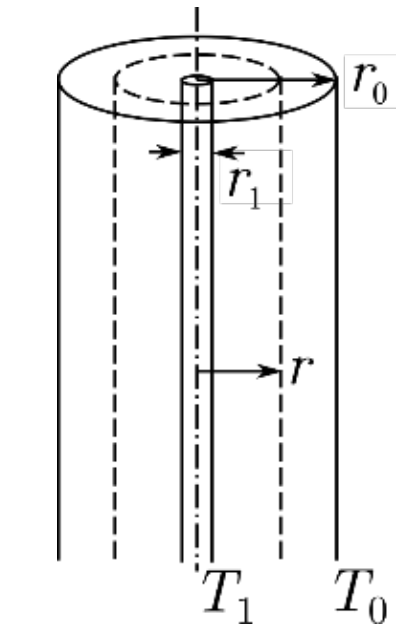
\includegraphics[width=0.2\textwidth]{1.png}
    \caption{Геометрия задачи}
    \label{fig:1}
\end{figure}
В таком случае закон Фурье(\ref{eq:1}) принимает вид:
\begin{equation}
    q = -\kappa \frac{dT}{dr}.
    \label{eq:3}
\end{equation}
Тогда поток тепла $Q$ через всю поверхность:
\begin{equation}
    Q = -2\pi L \cdot \kappa \frac{dT}{dr}.
    \label{eq:4}
\end{equation}
Пренебрегая зависимостью теплоёмкости от температуры для небольших $\Delta T$, проинтегрируем выражение \ref{eq:4}:
\begin{equation}
    Q = \frac{2\pi L}{\ln \frac{r_0}{r_1}} \kappa \Delta T
    \label{eq:QdT}
\end{equation}

\subsection{Проведение эксперимента}
Экспериментальная установка (Рис. \ref{fig:2}) представляет собой 
циллиндрическую трубку заполненную воздухом с проведённом металлической нитью внутри.
Температура внешних стенок $t_0$ 
поддерживается постоянной при помощи циркулирующей через стенки жидкости.
\begin{figure}[H]
    \centering
    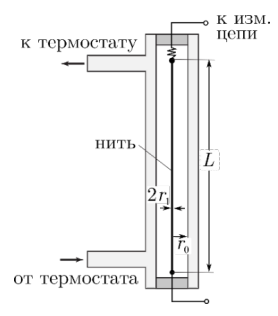
\includegraphics[width=0.3\textwidth]{2.png}
    \caption{Схема установки}
    \label{fig:2}
\end{figure} 
Нить разогревается при пропускании через неё постоянного тока $I$.
Подводимую мощность $Q$  можно расчитать измеряя ток $I$ и напряжение $U$ на нити как
\begin{equation}
    Q = UI.
    \label{eq:6}
\end{equation}
При этом сопротивление нити $R$ вычисляется как
\begin{equation}
    R = \frac{U}{I}
    \label{eq:7}
\end{equation}  
Так как сопротивление нити однозначно определяется её температурой, зная зависимость $R(t)$ можно найти температуру нагревателя $t_1$ . 
Известно, что в исследуемом диапазоне температур таккая зависимость выражается через температуру как
\begin{equation}
    R = R_{273} (1 + \alpha T), 
    \label{eq:RT}
\end{equation}
где $t$ - температура в [\textcelsius], $R_{273}$ - сопротивление нити при температуре $0$ \textcelsius, 
$\alpha = \frac{1}{R_{273}}\frac{dR}{dT}$ - температурный коэффициент сопротивления материала. 
Тогда измерив нагрузочные кривые $R(Q)$ при различных $t_0$ и аппроксимируя их при значении $Q \to 0$ получим 
значение сопротивления $R$ от температуры $t_0$. Построив зависимость $R(t_0)$ найдём коэффициент $\frac{dR}{dT}$. И тогда 
найдём $\frac{2\pi L}{\ln \frac{r_0}{r_1}} \kappa = \frac{d Q}{d (\Delta T)} = \frac{d R}{d T} / \frac{d R}{d Q}$      

\section{Результаты и их обсуждение}
Для каждой из температур термостата измерены зависимости напряжения \(U\) и силы тока \(I\) на нагрузке \(R_n\) (Приложение \ref{app_2}, Таблицы \ref{tab:1} - \ref{tab:7}).
Рассчитаны зависимости сопротивления нагрузки \(R_n = \frac{U}{I}\) от мощности, выделяемой на ней \(Q = UI\).
Для каждой из температур из графиков зависимости сопротивления нагрузки \(R_n(Q)\) (Рис. \ref{fig:RQ}) определёны коэффициенты наклона нагрузочных кривых \(\beta = \frac{d R}{d Q}\) и 
температуры нагрузки при температуре термостата \(R_0\) (Таблица \ref{tab:RT}).
Зависимости \(R_n(Q)\) оказались линейными, что даёт подтверждение корректности используемой модели.
\begin{figure}[H]
    \centering
    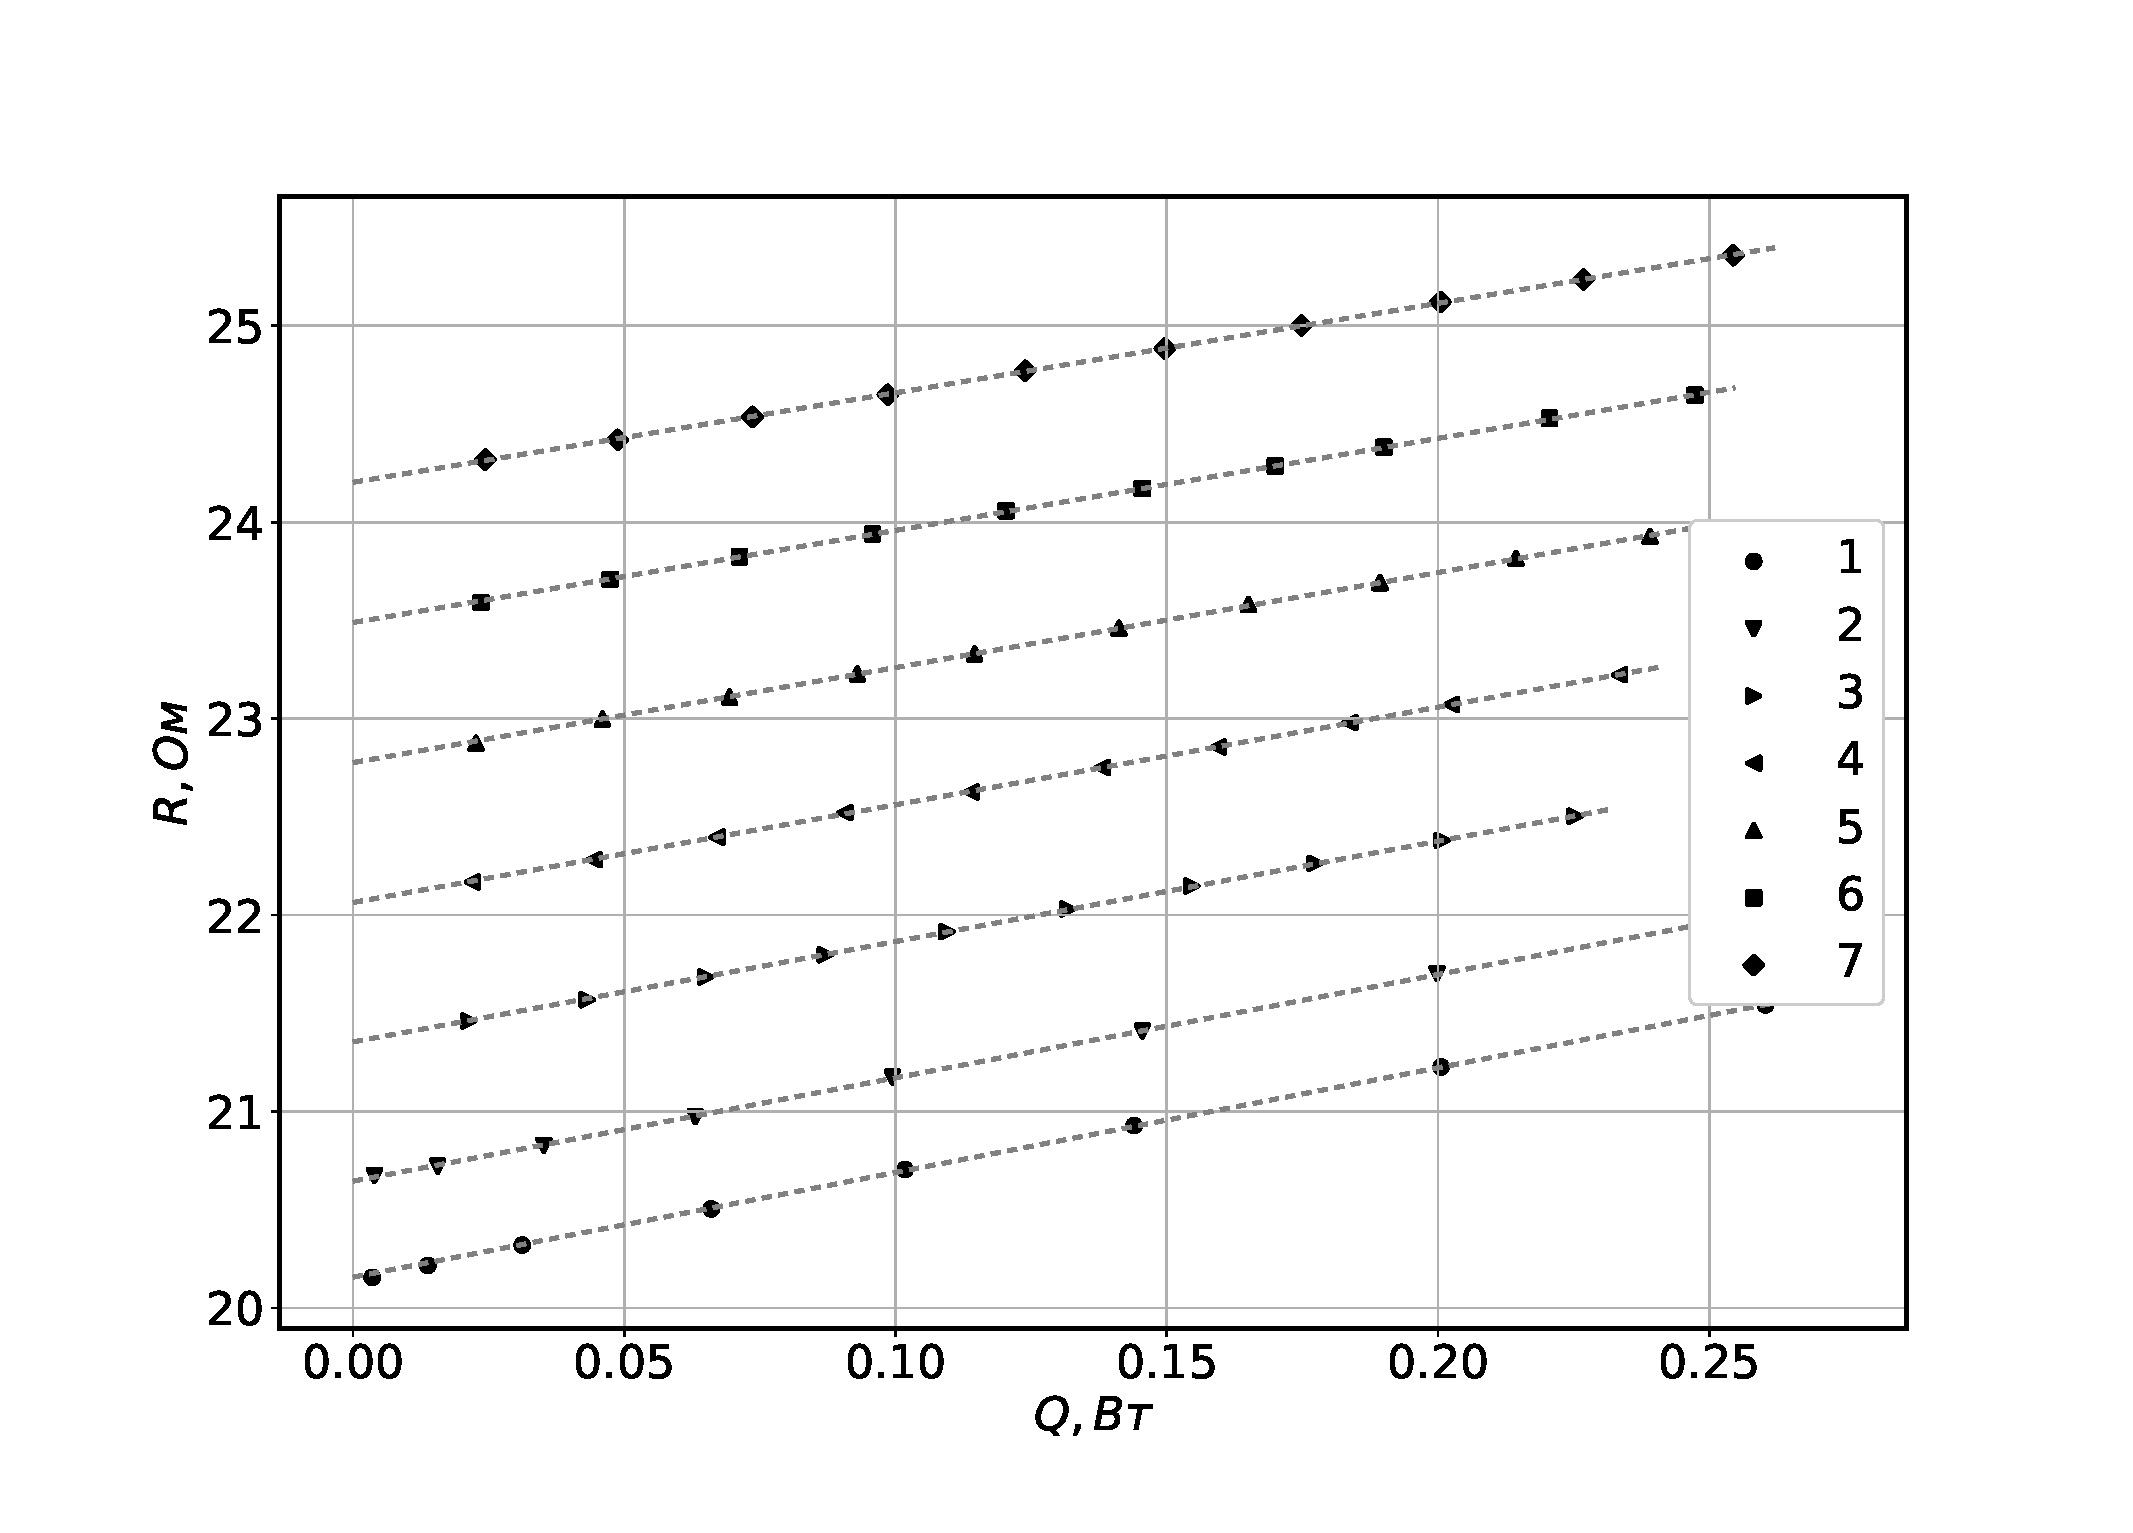
\includegraphics[width=0.8\textwidth]{RQ.eps}
    \caption{Зависимость сопротивления нагрузки \(R_n\) от мощности \(Q\), выделяющеейся на ней, при различных температурах.
        Цифрами обозначены данные для каждой из температур: 
        1 - \(23\) \textcelsius, 2 - \(30\) \textcelsius, 3 - \(40\) \textcelsius, 4 - \(50\) \textcelsius, 5 - \(60\) \textcelsius, 6 - \(70\) \textcelsius, 7 - \(80\) \textcelsius. Кресты погрешности малы по сравнению с масштабом графика и потому не были нанесены.      }
    \label{fig:RQ}
\end{figure}
Построены графики зависимости сопротивления нагрузки \(R_0\) от температуры \(T\) (Рис. \ref{fig:RT}). Полученный зависимость оказалась линейной, что подтверждает корректность 
использования формулы \ref{eq:RT}.
\begin{figure}[H]
    \centering
    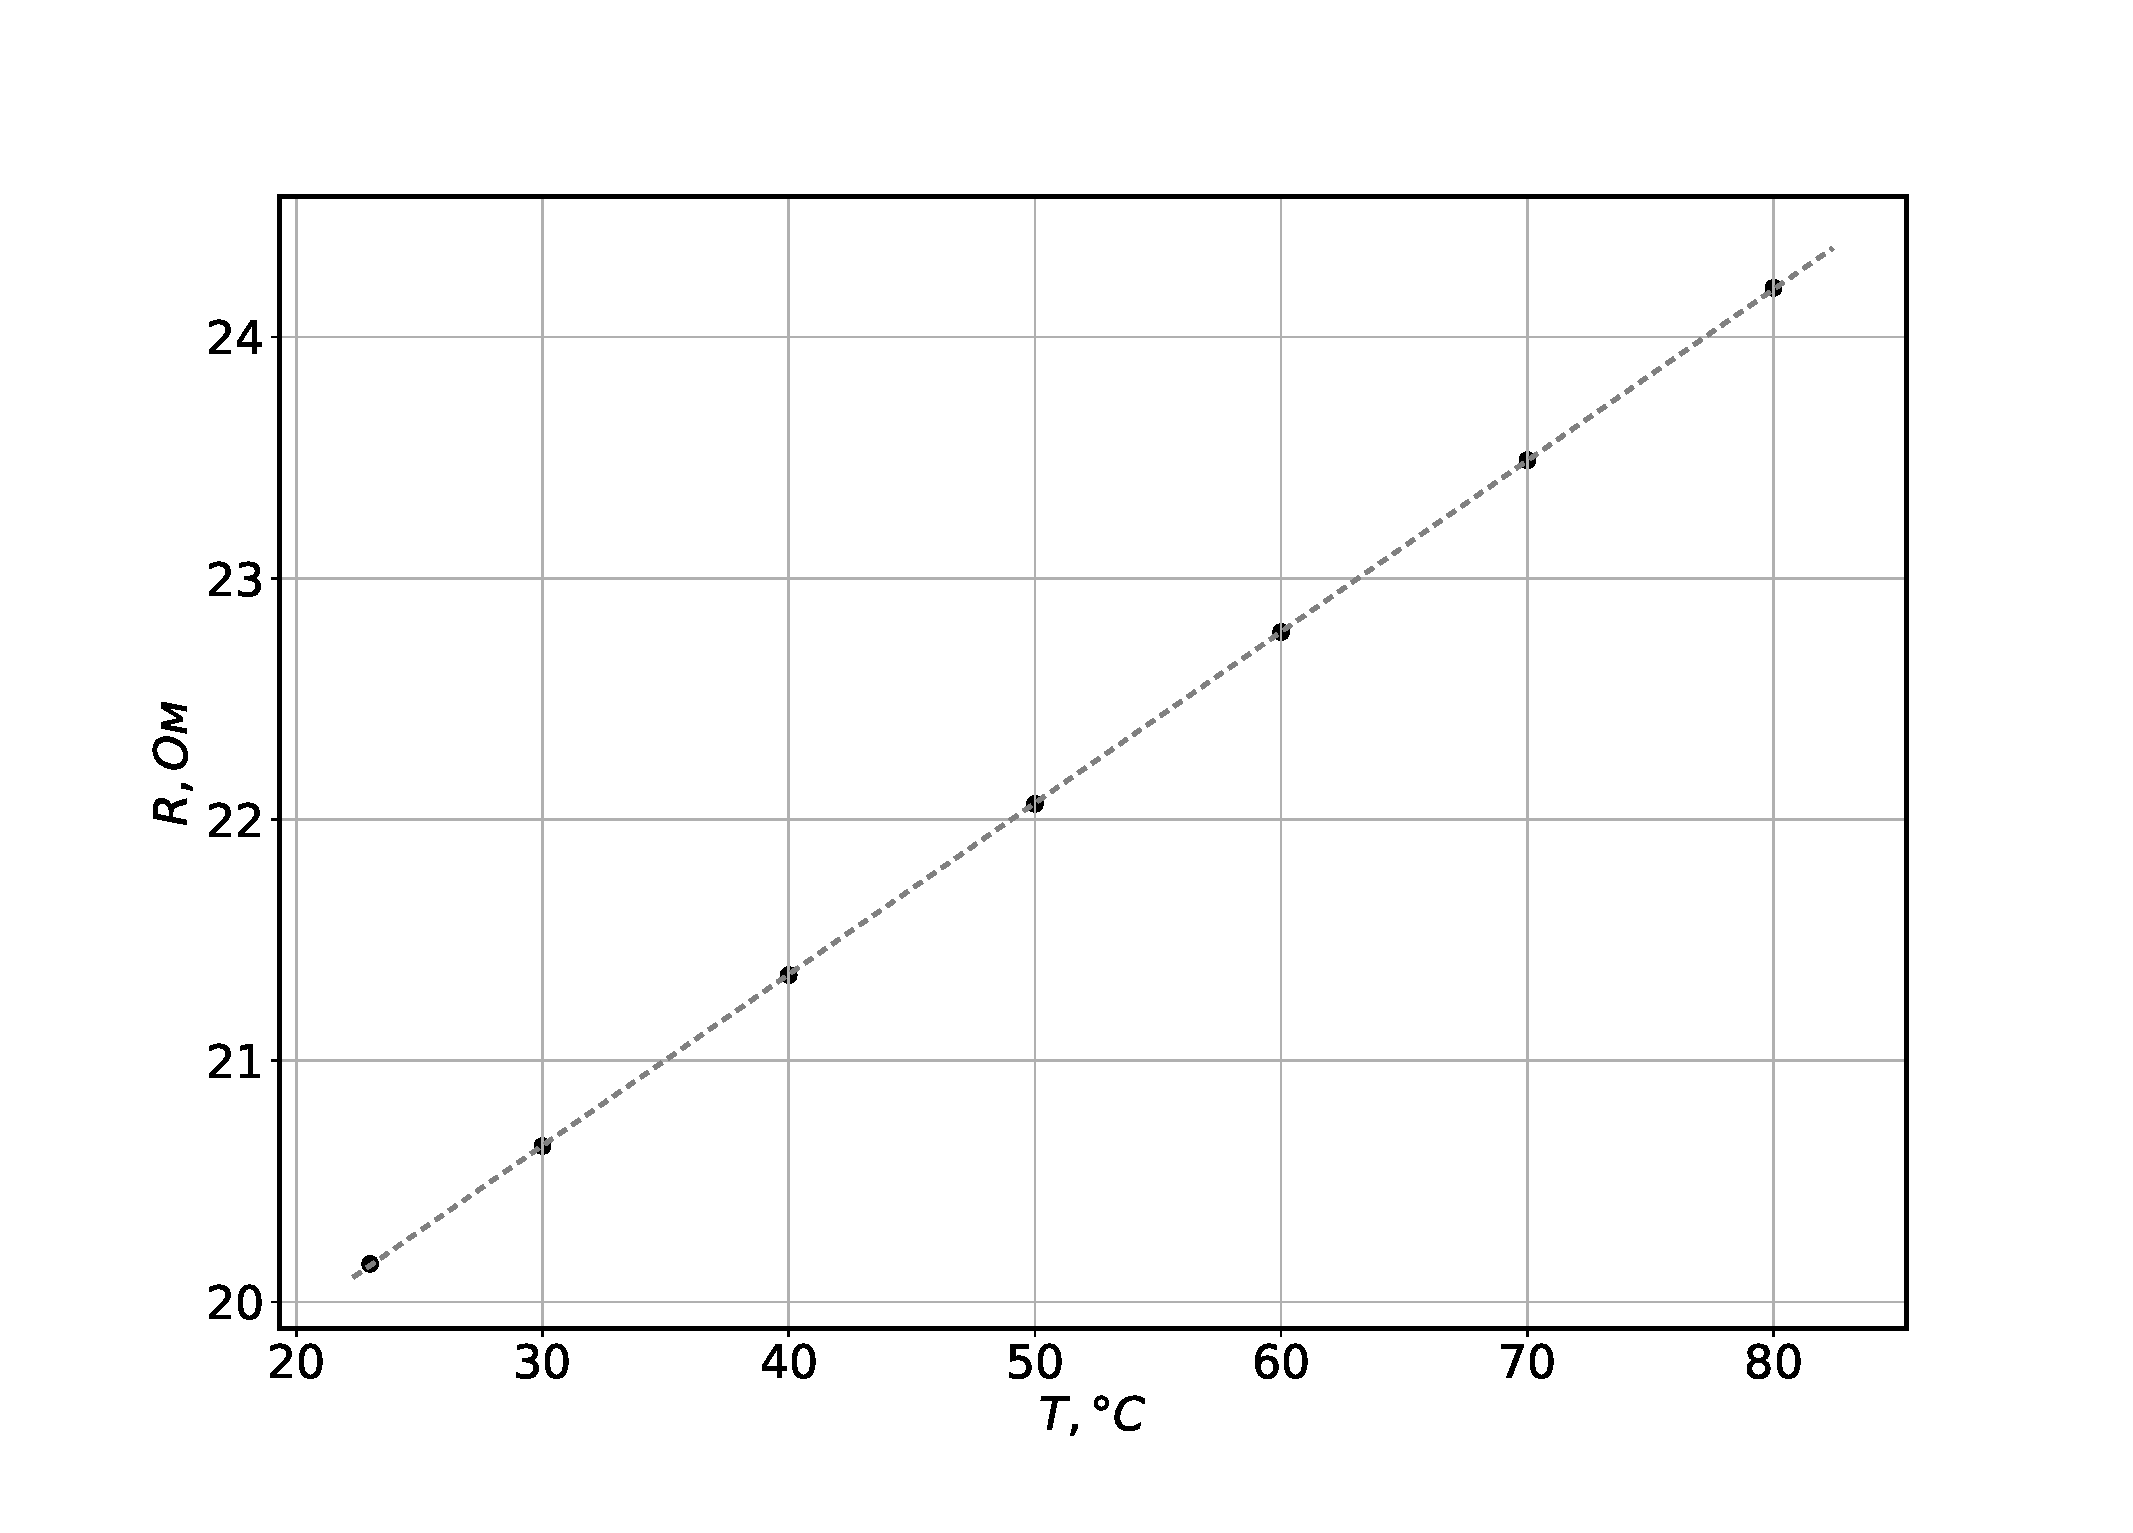
\includegraphics[width=0.8\textwidth]{RT.eps}
    \caption{Зависимость сопротивления нагрузки \(R_0\) от температуры \(T\). Кресты погрешности малы по сравнению с масштабом графика и потому не были нанесены.}
    \label{fig:RT}
\end{figure}
Рассчитаны сопротивление нагрузки \(R_{273} = (1.852 \pm 0.004) \cdot 10 ^ {1}\) Ом и температурный коэффициент сопротивления материала 
\(\alpha = (3.836 \pm 0.009) \cdot 10 ^ {-3} \) \(\frac{1}{\textrm{\textcelsius}}\).
Согласно формуле \ref{eq:QdT} найдено значение теплопроводности для различных температур (Таблица \ref{tab:kappaT}), где \(\frac{d Q}{d (\Delta T)} = \frac{d R}{d T} / \frac{d R}{d Q}\).
С учётом предположенной зависимости, имеющий вид \(\kappa = A T^{n} \) построим логарифмическую зависимость \(\ln \kappa = n \ln T + \ln A\) (Рис. \ref{fig:lnkT}).   
\begin{figure}[H]
    \centering
    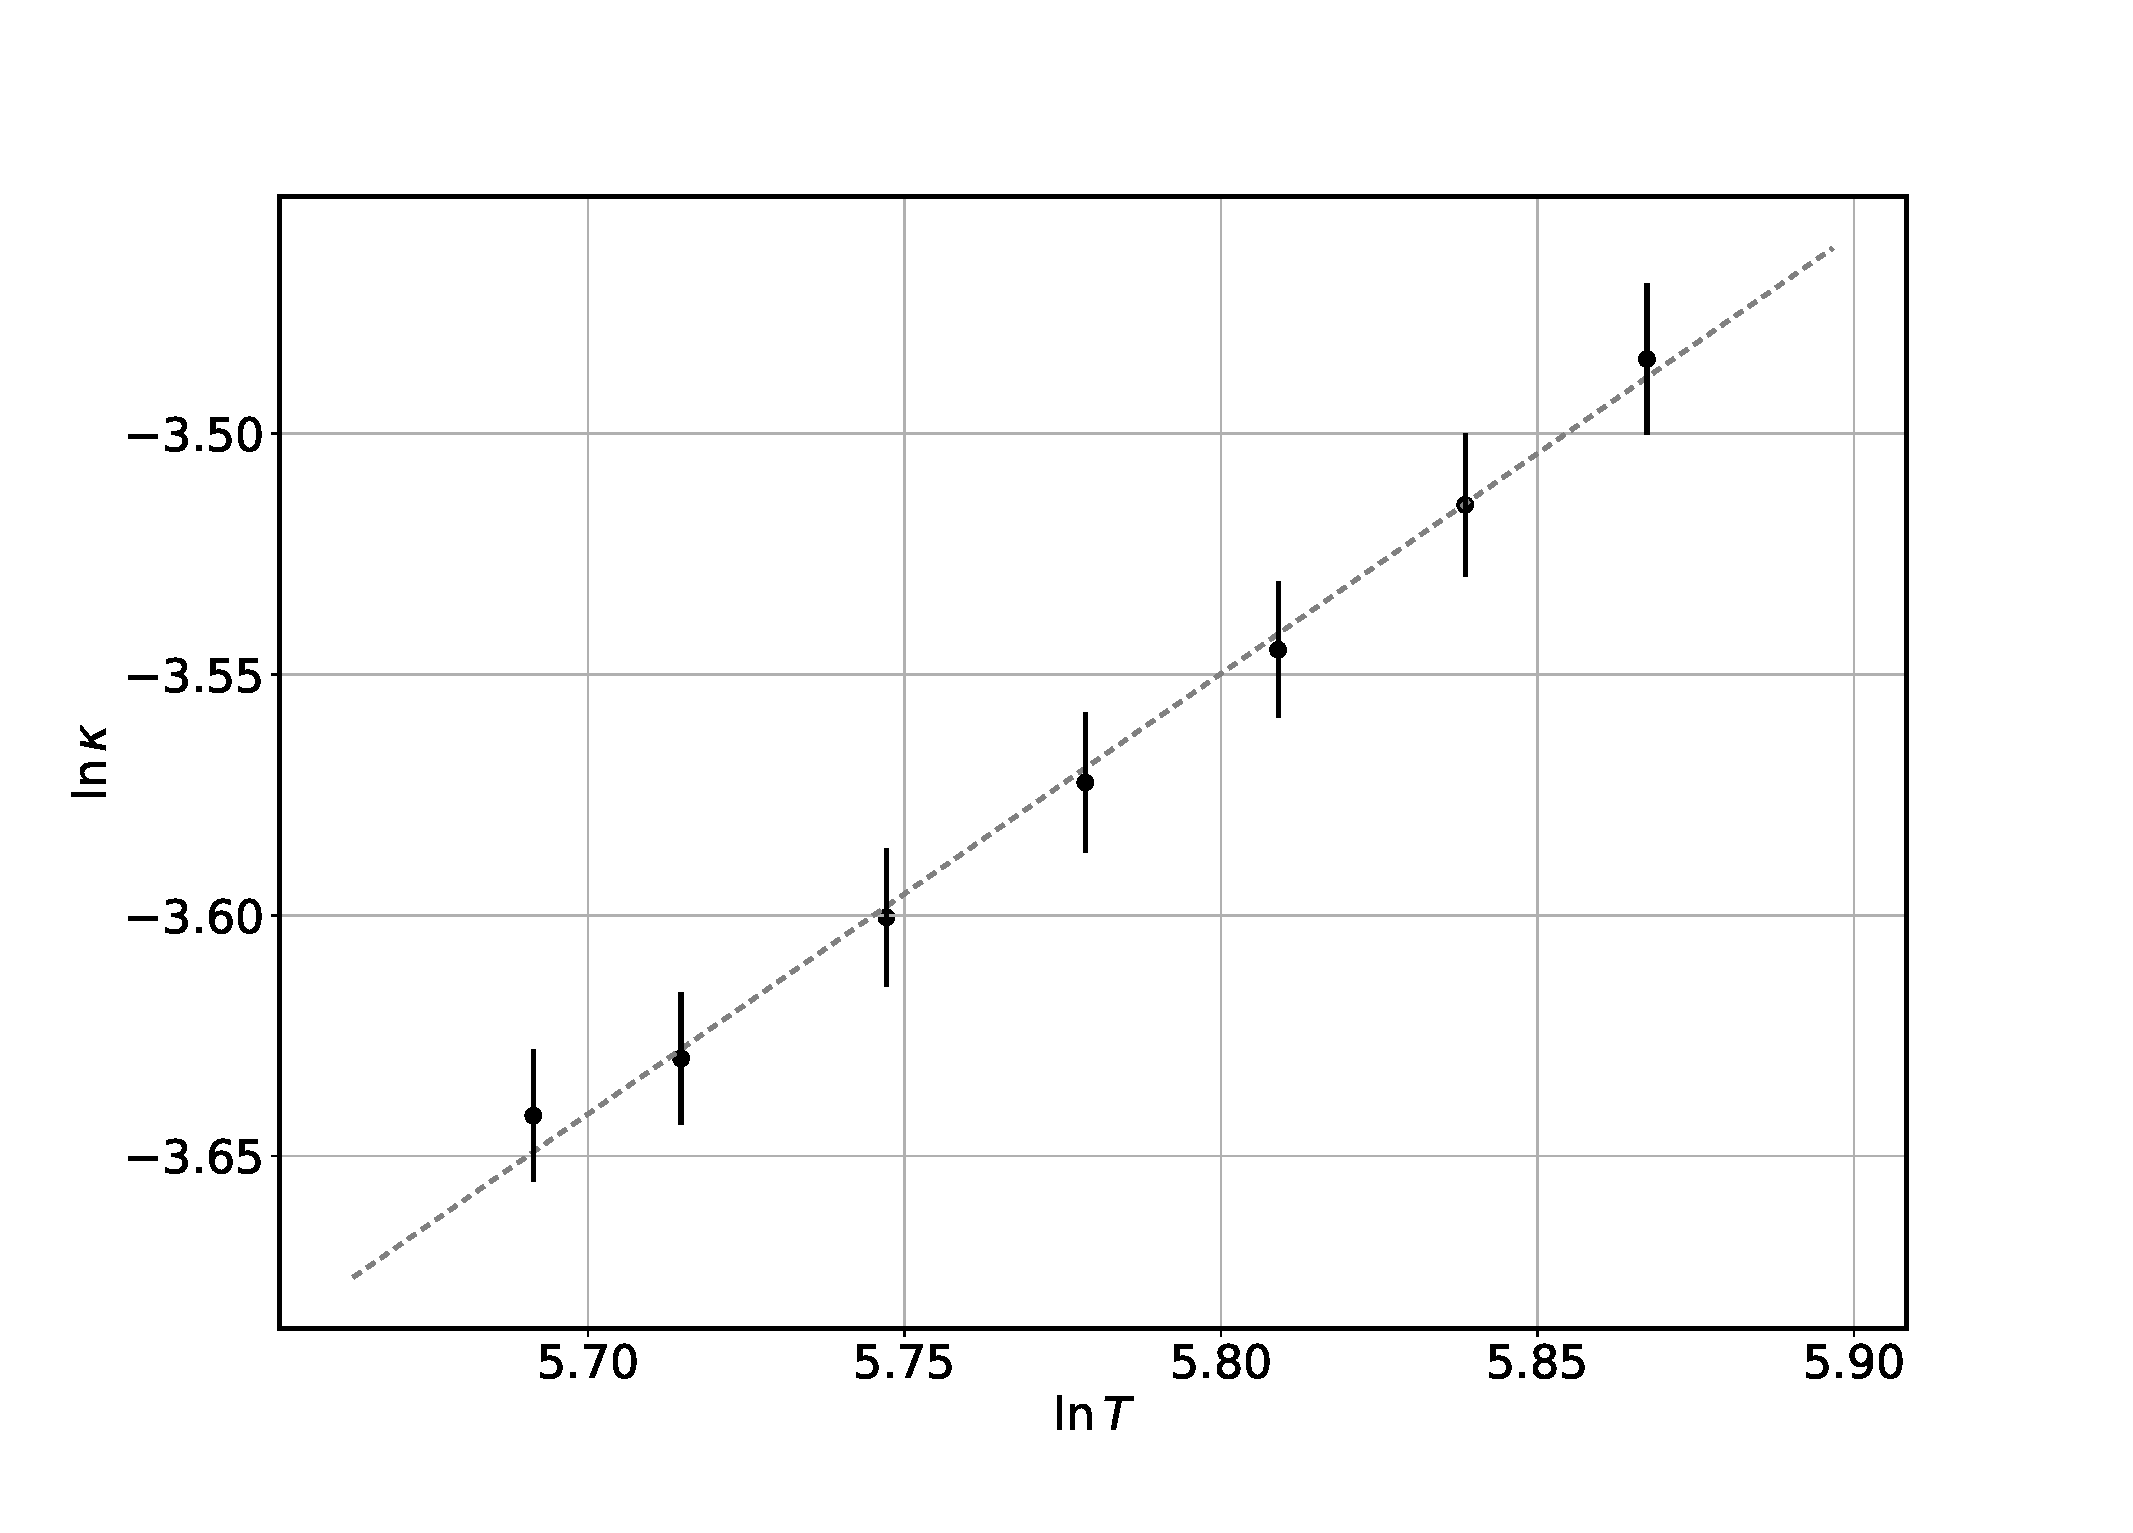
\includegraphics[width=0.8\textwidth]{lnkT.eps}
    \caption{Зависимость коэффициента теплопроводности воздуха \(\kappa \) от абсолютной температуры \(T\) в логарифмическом масштабе.}
    \label{fig:lnkT}
\end{figure}
Полученные коэффициенты оказались равны \(\ln A = (-8.85 \pm 0.38)\), \(n = (9.15 \pm 0.37) \cdot 10 ^ {-1} \approx 1\). По полученным значениям 
построим график зависимости \(\kappa (T)\) (Рис. \ref{fig:kT}).  
\begin{figure}[H]
    \centering
    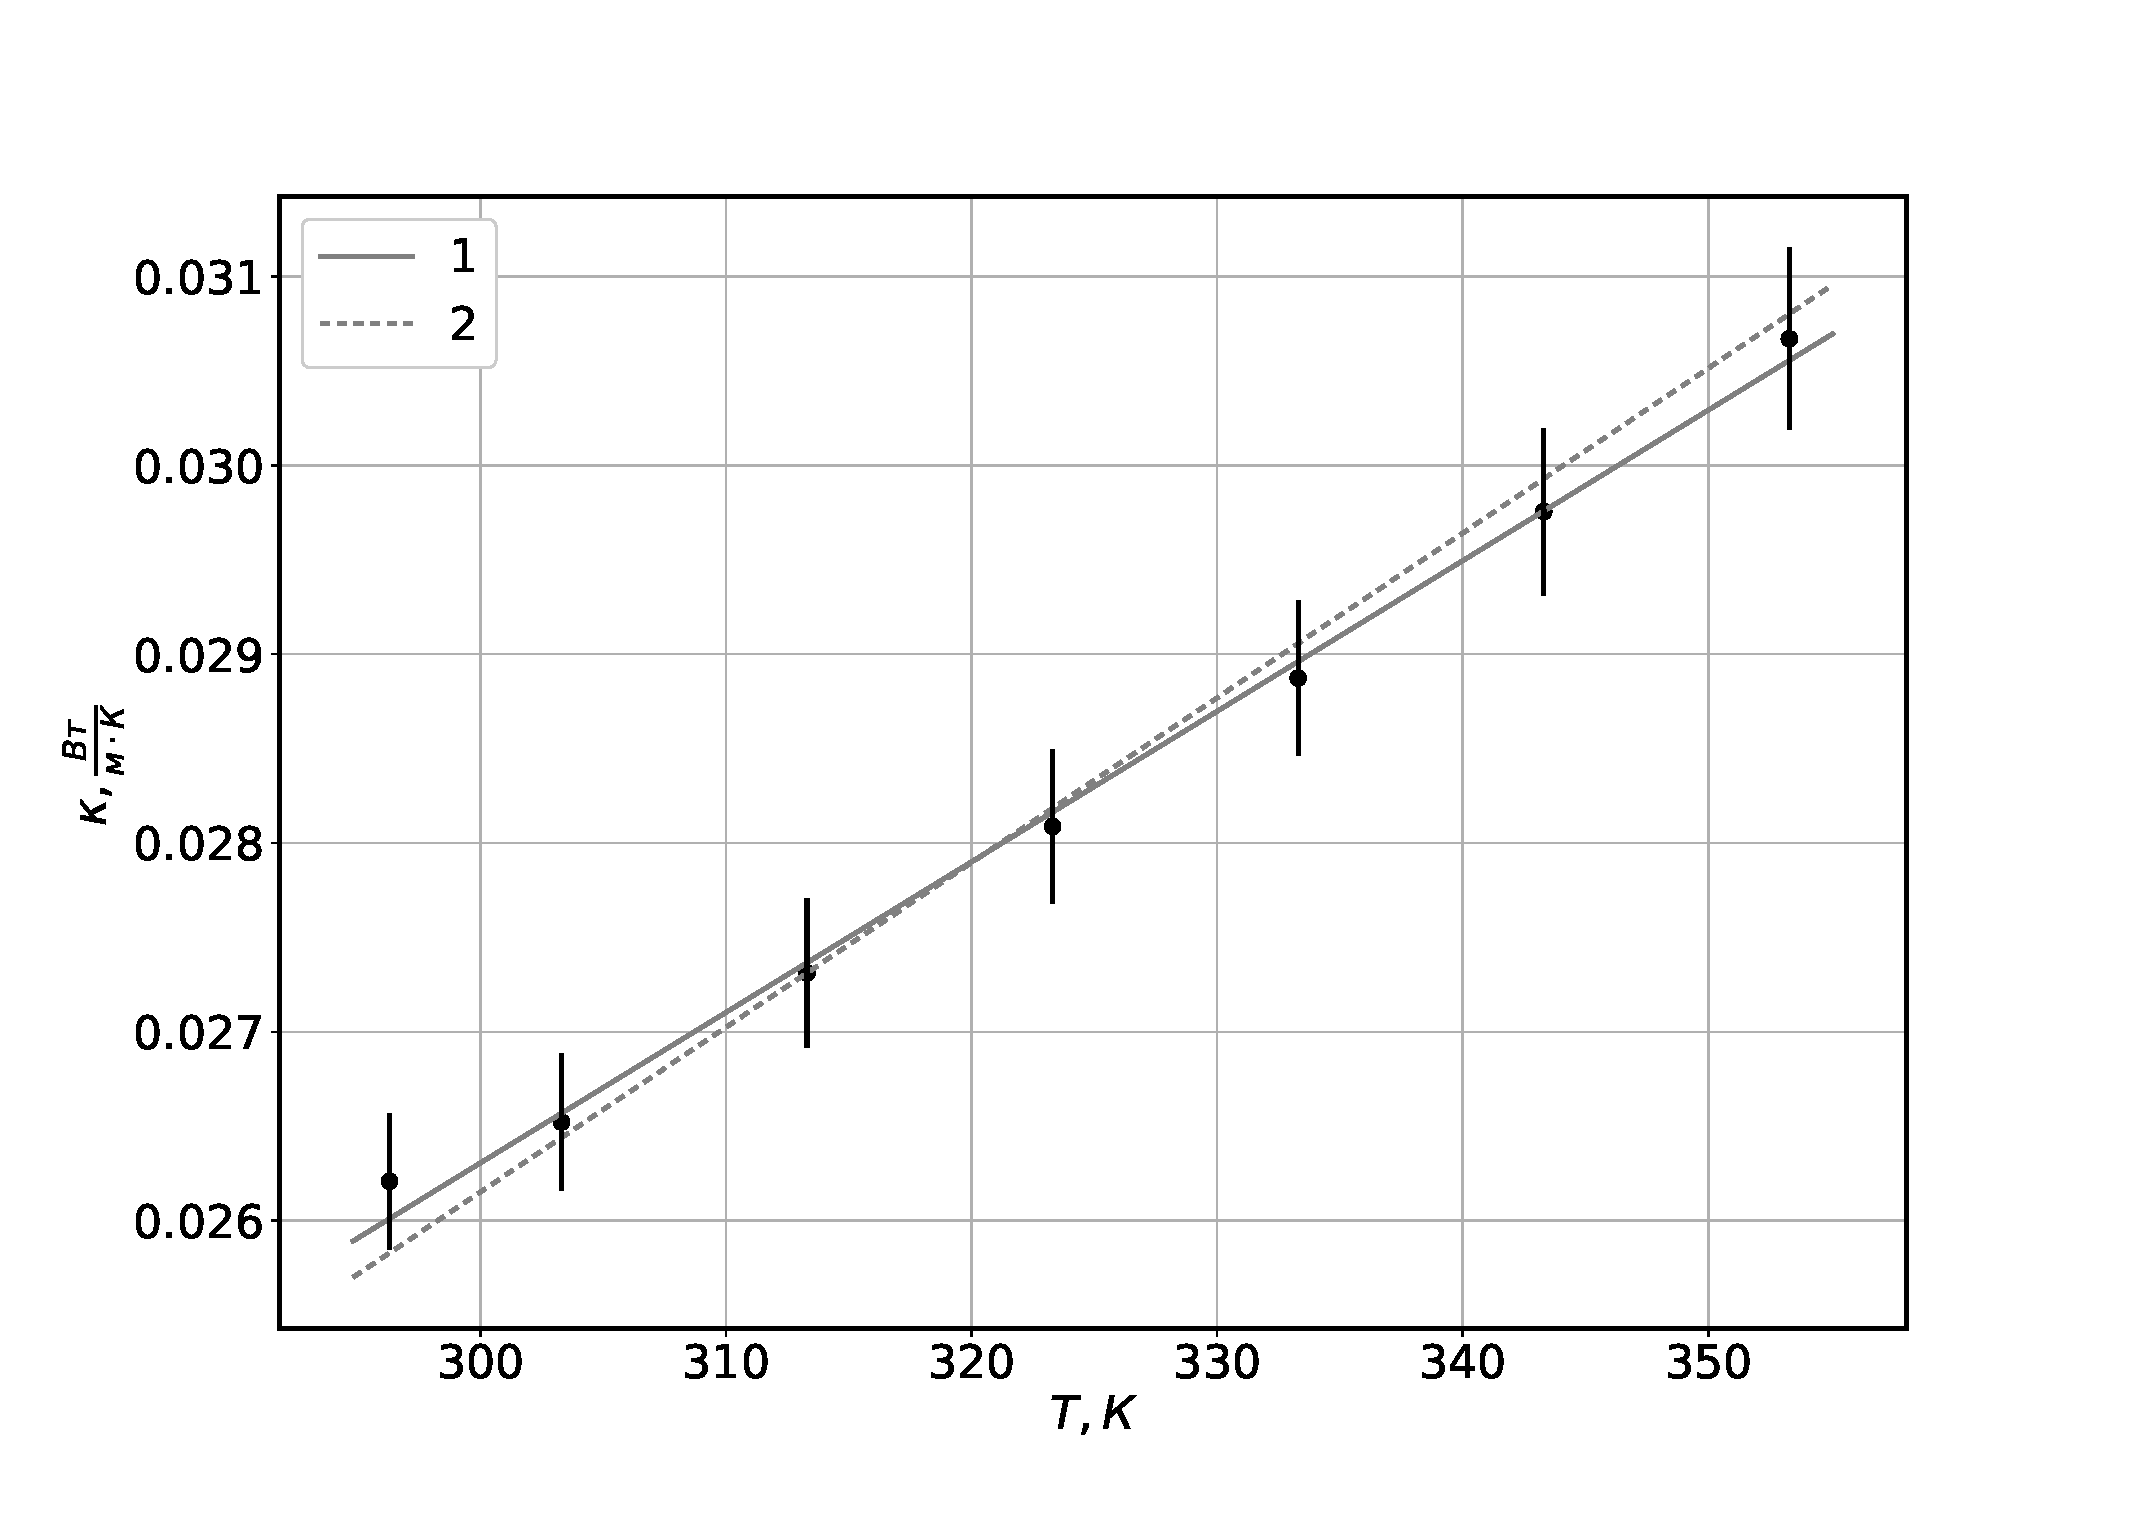
\includegraphics[width=0.8\textwidth]{kT.eps}
    \caption{Зависимость коэффициента теплопроводности воздуха \(\kappa \) от абсолютной температуры \(T\). Цифрами обозначены кривые, аппроксимирующие
        зависимость: 1 - \(\kappa = A T^n\), 2 - \(\kappa = A T\).}
    \label{fig:kT}
\end{figure}

Оказалось, что зависимость коэффициента теплопроводности от температуры близка к линейной, что разходится с теорией
твёрдых шариков, где предсказывается зависимость, пропорциональная квадратному корню из температуры. 
Такое расхождение может объясняться малым диапазоном измерения температур или несовершенством модели.

\section{Выводы}
Найдены значения коэффициентов теплопроводности воздуха в диапазоне \(20 - 80\) \textcelsius. Определён 
экспериментальный вид зависимости коэффициента теплопроводности воздуха от температуры, вблизи указанного 
диапазона температур \(\kappa = A T\), где \(A = (8.714 \pm 0.024) \cdot 10 ^ {-5}\) \(\frac{\textrm{Вт}}{\textrm{м} \cdot \textrm{К}^2}\).

\section{Использованная литература}
\begin{thebibliography}{9}
    \bibitem{LabBook}
    Лабораторный практикум по общей физике, Том 1, под редакцией А. Д. Гладуна
    \bibitem{Kirichenko}
    Н.А. Кириченко «Термодинамика, статистическая и молекулярная физика», п. 5.5
\end{thebibliography}

\section{Приложения}
\subsection{Параметры установки и погрешности приборов} \label{app_1}
Внутренний диаметр \(d_1 = (5.0 \pm 0.3) \cdot 10 ^ {-5}\) м, внешний диаметр \(d_2 = (7.00 \pm 0.10) \cdot 10 ^ {-3}\) м, длина установки \(L = (4.000 \pm 0.020) \cdot 10 ^ {-1}\) м. 
Погрешности измерения амперметра и вольтметра взяты за последнюю цифру измерения, значение которой 
стабилизировалось при измерениях: \(\sigma  U = 10^{-4}\) В, \(\sigma I = 10^{-5}\) А.
\subsection{Данные результатов измерений} \label{app_2}
\begin{table}[H]
    \centering
    \begin{tabular}{|l|l|l|l|l|l|l|}
        \hline
          & $U$, В & $I$, A  & $Q$, Вт & $R$, Ом & $\sigma Q$, Вт $\cdot 10^{-6}$ & $\sigma R$, Ом \\
        \hline
        0 & 0.2658 & 0.01319 & 0.00351 & 20.156  & 3.0                            & 0.017          \\
        1 & 0.5277 & 0.02610 & 0.01377 & 20.217  & 6.0                            & 0.009          \\
        2 & 0.7959 & 0.03917 & 0.03117 & 20.320  & 9.0                            & 0.006          \\
        3 & 1.1636 & 0.05675 & 0.06603 & 20.505  & 13                             & 0.004          \\
        4 & 1.4514 & 0.07010 & 0.10174 & 20.705  & 16                             & 0.003          \\
        5 & 1.7358 & 0.08294 & 0.14397 & 20.928  & 19                             & 0.003          \\
        6 & 2.0635 & 0.09721 & 0.20059 & 21.227  & 23                             & 0.002          \\
        7 & 2.3684 & 0.10994 & 0.26038 & 21.543  & 26                             & 0.002          \\
        \hline
    \end{tabular}
    
    \caption{Результаты измерений сопростивления \(R\) от выделяемого тепла \(Q\) при температуре \(T = 23\)\textcelsius.
        Прямыми измерениями являются напряжение \(U\) и ток \(I\), \(\sigma Q\) и \(\sigma R\) - погрешности косвенных измерений.}
    \label{tab:1}
\end{table}
\begin{table}[H]
    \centering
    \begin{tabular}{|l|l|l|l|l|l|l|}
        \hline
          & $U$, В & $I$, A  & $Q$, Вт & $R$, Ом & $\sigma Q$, Вт $\cdot 10^{-6}$ & $\sigma R$, Ом \\
        \hline
        0 & 0.2849 & 0.01378 & 0.00393 & 20.675  & 3.0                            & 0.017          \\
        1 & 0.5684 & 0.02743 & 0.01559 & 20.722  & 6.0                            & 0.008          \\
        2 & 0.8556 & 0.04108 & 0.03515 & 20.828  & 9.0                            & 0.006          \\
        3 & 1.1502 & 0.05484 & 0.06308 & 20.974  & 13                             & 0.004          \\
        4 & 1.4509 & 0.06852 & 0.09942 & 21.175  & 16                             & 0.003          \\
        5 & 1.7650 & 0.08244 & 0.14551 & 21.410  & 19                             & 0.003          \\
        6 & 2.0824 & 0.09595 & 0.19981 & 21.703  & 23                             & 0.002          \\
        7 & 2.4158 & 0.10962 & 0.26482 & 22.038  & 27                             & 0.002          \\
        \hline
    \end{tabular}
    
    \caption{Результаты измерений сопростивления \(R\) от выделяемого тепла \(Q\) при температуре \(T = 30\)\textcelsius.
        Прямыми измерениями являются напряжение \(U\) и ток \(I\), \(\sigma Q\) и \(\sigma R\) - погрешности косвенных измерений.}
    \label{tab:2}
\end{table}
\begin{table}[H]
    \centering
    \begin{tabular}{|l|l|l|l|l|l|l|}
        \hline
          & $U$, В & $I$, A  & $Q$, Вт & $R$, Ом & $\sigma Q$, Вт $\cdot 10^{-6}$ & $\sigma R$, Ом \\
        \hline
        0 & 0.6760 & 0.03150 & 0.02129 & 21.460  & 7.0                            & 0.008          \\
        1 & 0.9648 & 0.04473 & 0.04316 & 21.569  & 11                             & 0.005          \\
        2 & 1.1871 & 0.05474 & 0.06498 & 21.686  & 13                             & 0.004          \\
        3 & 1.3774 & 0.06319 & 0.08704 & 21.798  & 15                             & 0.004          \\
        4 & 1.5488 & 0.07067 & 0.10945 & 21.916  & 17                             & 0.003          \\
        5 & 1.7034 & 0.07732 & 0.13171 & 22.031  & 19                             & 0.003          \\
        6 & 1.8505 & 0.08355 & 0.15461 & 22.148  & 20                             & 0.003          \\
        7 & 1.9870 & 0.08925 & 0.17734 & 22.263  & 22                             & 0.003          \\
        8 & 2.1199 & 0.09472 & 0.2008  & 22.381  & 23                             & 0.003          \\
        9 & 2.2515 & 0.10005 & 0.22526 & 22.504  & 25                             & 0.002          \\
        \hline
    \end{tabular}
    
    \caption{Результаты измерений сопростивления \(R\) от выделяемого тепла \(Q\) при температуре \(T = 40\)\textcelsius.
        Прямыми измерениями являются напряжение \(U\) и ток \(I\), \(\sigma Q\) и \(\sigma R\) - погрешности косвенных измерений.}
    \label{tab:3}
\end{table}
\begin{table}[H]
    \centering
    \begin{tabular}{|l|l|l|l|l|l|l|}
        \hline
          & $U$, В & $I$, A  & $Q$, Вт & $R$, Ом & $\sigma Q$, Вт $\cdot 10^{-6}$ & $\sigma R$, Ом \\
        \hline
        0 & 0.6981 & 0.03149 & 0.02198 & 22.169  & 8.0                            & 0.008          \\
        1 & 0.9949 & 0.04465 & 0.04442 & 22.282  & 11                             & 0.005          \\
        2 & 1.2258 & 0.05473 & 0.06709 & 22.397  & 13                             & 0.004          \\
        3 & 1.4288 & 0.06344 & 0.09064 & 22.522  & 16                             & 0.004          \\
        4 & 1.6056 & 0.07096 & 0.11393 & 22.627  & 18                             & 0.003          \\
        5 & 1.7726 & 0.07791 & 0.13810 & 22.752  & 19                             & 0.003          \\
        6 & 1.9092 & 0.08353 & 0.15948 & 22.856  & 21                             & 0.003          \\
        7 & 2.0549 & 0.08942 & 0.18375 & 22.98   & 22                             & 0.003          \\
        8 & 2.1616 & 0.09369 & 0.20252 & 23.072  & 24                             & 0.003          \\
        9 & 2.3284 & 0.10026 & 0.23345 & 23.224  & 25                             & 0.003          \\
        \hline
    \end{tabular}
    
    \caption{Результаты измерений сопростивления \(R\) от выделяемого тепла \(Q\) при температуре \(T = 50\)\textcelsius.
        Прямыми измерениями являются напряжение \(U\) и ток \(I\), \(\sigma Q\) и \(\sigma R\) - погрешности косвенных измерений.}
    \label{tab:4}
\end{table}
\begin{table}[H]
    \centering
    \begin{tabular}{|l|l|l|l|l|l|l|}
        \hline
          & $U$, В & $I$, A  & $Q$, Вт & $R$, Ом & $\sigma Q$, Вт $\cdot 10^{-6}$ & $\sigma R$, Ом \\
        \hline
        0 & 0.7199 & 0.03147 & 0.02266 & 22.876  & 8.0                            & 0.008          \\
        1 & 1.0280 & 0.04470 & 0.04595 & 22.998  & 11                             & 0.006          \\
        2 & 1.2664 & 0.05480 & 0.06940 & 23.109  & 14                             & 0.005          \\
        3 & 1.4694 & 0.06326 & 0.09295 & 23.228  & 16                             & 0.004          \\
        4 & 1.6349 & 0.07008 & 0.11457 & 23.329  & 18                             & 0.004          \\
        5 & 1.8201 & 0.07758 & 0.14120 & 23.461  & 20                             & 0.003          \\
        6 & 1.9728 & 0.08366 & 0.16504 & 23.581  & 21                             & 0.003          \\
        7 & 2.1178 & 0.08939 & 0.18931 & 23.692  & 23                             & 0.003          \\
        8 & 2.2594 & 0.09487 & 0.21435 & 23.816  & 25                             & 0.003          \\
        9 & 2.3919 & 0.09996 & 0.23909 & 23.929  & 26                             & 0.003          \\
        \hline
    \end{tabular}
    
    \caption{Результаты измерений сопростивления \(R\) от выделяемого тепла \(Q\) при температуре \(T = 60\)\textcelsius.
        Прямыми измерениями являются напряжение \(U\) и ток \(I\), \(\sigma Q\) и \(\sigma R\) - погрешности косвенных измерений.}
    \label{tab:5}
\end{table}
\begin{table}[H]
    \centering
    \begin{tabular}{|l|l|l|l|l|l|l|}
        \hline
          & $U$, В & $I$, A  & $Q$, Вт & $R$, Ом & $\sigma Q$, Вт $\cdot 10^{-6}$ & $\sigma R$, Ом \\
        \hline
        0 & 0.7457 & 0.03161 & 0.02357 & 23.591  & 8.0                            & 0.008          \\
        1 & 1.0598 & 0.04470 & 0.04737 & 23.709  & 12                             & 0.006          \\
        2 & 1.3027 & 0.05468 & 0.07123 & 23.824  & 14                             & 0.005          \\
        3 & 1.5142 & 0.06325 & 0.09577 & 23.940  & 16                             & 0.004          \\
        4 & 1.7019 & 0.07074 & 0.12039 & 24.059  & 18                             & 0.004          \\
        5 & 1.8752 & 0.07758 & 0.14548 & 24.171  & 20                             & 0.003          \\
        6 & 2.0318 & 0.08366 & 0.16998 & 24.286  & 22                             & 0.003          \\
        7 & 2.1524 & 0.08828 & 0.19001 & 24.382  & 23                             & 0.003          \\
        8 & 2.3261 & 0.09483 & 0.22058 & 24.529  & 25                             & 0.003          \\
        9 & 2.4691 & 0.10018 & 0.24735 & 24.647  & 27                             & 0.003          \\
        \hline
    \end{tabular}
    
    \caption{Результаты измерений сопростивления \(R\) от выделяемого тепла \(Q\) при температуре \(T = 70\)\textcelsius.
        Прямыми измерениями являются напряжение \(U\) и ток \(I\), \(\sigma Q\) и \(\sigma R\) - погрешности косвенных измерений.}
    \label{tab:6}
\end{table}
\begin{table}[H]
    \centering
    \begin{tabular}{|l|l|l|l|l|l|l|}
        \hline
          & $U$, В & $I$, A  & $Q$, Вт & $R$, Ом & $\sigma Q$, Вт $\cdot 10^{-6}$ & $\sigma R$, Ом \\
        \hline
        0 & 0.7697 & 0.03165 & 0.02436 & 24.319  & 8.0                            & 0.008          \\
        1 & 1.0913 & 0.04469 & 0.04877 & 24.419  & 12                             & 0.006          \\
        2 & 1.3441 & 0.05478 & 0.07363 & 24.536  & 15                             & 0.005          \\
        3 & 1.5588 & 0.06324 & 0.09858 & 24.649  & 17                             & 0.004          \\
        4 & 1.7518 & 0.07072 & 0.12389 & 24.771  & 19                             & 0.004          \\
        5 & 1.9298 & 0.07755 & 0.14966 & 24.885  & 21                             & 0.003          \\
        6 & 2.0909 & 0.08363 & 0.17486 & 25.002  & 23                             & 0.003          \\
        7 & 2.2438 & 0.08932 & 0.20042 & 25.121  & 24                             & 0.003          \\
        8 & 2.3926 & 0.09481 & 0.22684 & 25.236  & 26                             & 0.003          \\
        9 & 2.5402 & 0.10017 & 0.25445 & 25.359  & 27                             & 0.003          \\
        \hline
    \end{tabular}
    
    \caption{Результаты измерений сопростивления \(R\) от выделяемого тепла \(Q\) при температуре \(T = 80\)\textcelsius.
        Прямыми измерениями являются напряжение \(U\) и ток \(I\), \(\sigma Q\) и \(\sigma R\) - погрешности косвенных измерений.}
    \label{tab:7}
\end{table}

\begin{table}[H]
    \centering
    \begin{tabular}{|l|l|l|l|l|l|}
        \hline
          & $T$, \textcelsius & $R_0$, Ом & $\beta$, $\frac{\textrm{Ом}}{\textrm{Вт}}$ & $\sigma R_0$, Ом & $\sigma \beta$, $\frac{\textrm{Ом}}{\textrm{Вт}}$ \\
        \hline
        0 & 23.0              & 20.157    & 5.33                                       & 0.003            & 0.01                                              \\
        1 & 30.0              & 20.646    & 5.27                                       & 0.003            & 0.01                                              \\
        2 & 40.0              & 21.355    & 5.11                                       & 0.004            & 0.02                                              \\
        3 & 50.0              & 22.064    & 4.97                                       & 0.004            & 0.03                                              \\
        4 & 60.0              & 22.777    & 4.84                                       & 0.004            & 0.02                                              \\
        5 & 70.0              & 23.489    & 4.69                                       & 0.005            & 0.03                                              \\
        6 & 80.0              & 24.203    & 4.55                                       & 0.007            & 0.04                                              \\
        \hline
    \end{tabular}
    
    \caption{Значения сопротивлений нагрузок \(R_0\) при температурах \(T\) и коэффициентов \(\beta = \frac{d R}{d Q}\).}
    \label{tab:RT}
\end{table}

\begin{table}[H]
    \centering
    \begin{tabular}{|l|l|l|l|l|l|l|l|}
        \hline
          & $T$, \textcelsius & $\kappa$, \(\frac{\textrm{Вт}}{\textrm{м} \cdot \textrm{К}}\) & $\sigma \kappa$, \(\frac{\textrm{Вт}}{\textrm{м} \cdot \textrm{К}}\) & $\ln T$ & $\sigma \ln T$ & $\ln \kappa$ & $\sigma \ln \kappa$ \\
        \hline
        0 & 23.0              & 0.0262                                                        & 0.0004                                                               & 5.6914  & 0.0003         & -3.64        & 0.01                \\
        1 & 30.0              & 0.0265                                                        & 0.0004                                                               & 5.7147  & 0.0003         & -3.63        & 0.01                \\
        2 & 40.0              & 0.0273                                                        & 0.0004                                                               & 5.7472  & 0.0003         & -3.60        & 0.01                \\
        3 & 50.0              & 0.0281                                                        & 0.0004                                                               & 5.7786  & 0.0003         & -3.57        & 0.01                \\
        4 & 60.0              & 0.0289                                                        & 0.0004                                                               & 5.8090  & 0.0003         & -3.54        & 0.01                \\
        5 & 70.0              & 0.0298                                                        & 0.0004                                                               & 5.8386  & 0.0003         & -3.51        & 0.01                \\
        6 & 80.0              & 0.0307                                                        & 0.0005                                                               & 5.8673  & 0.0003         & -3.48        & 0.02                \\
        \hline
    \end{tabular}
    \caption{Значения коэффициентов теплопроводности \(\kappa \) в зависимости от температуры \(T\).}
    \label{tab:kappaT}
\end{table}



\end{document}